%%%%%%%%%%%%%%%%%%%%%%%%%%%%%%%%%%%%%%%%%%%%%%%%%%%%%%%%%%%%%%%%%
% Lecture date: 20-01-20
%%%%%%%%%%%%%%%%%%%%%%%%%%%%%%%%%%%%%%%%%%%%%%%%%%%%%%%%%%%%%%%%%
\chapter{QCD and Proton Structure}
\section{Form Factor}
We use photon of momentum $q = k_i - k_f$ to look at proton.
\begin{align*}
   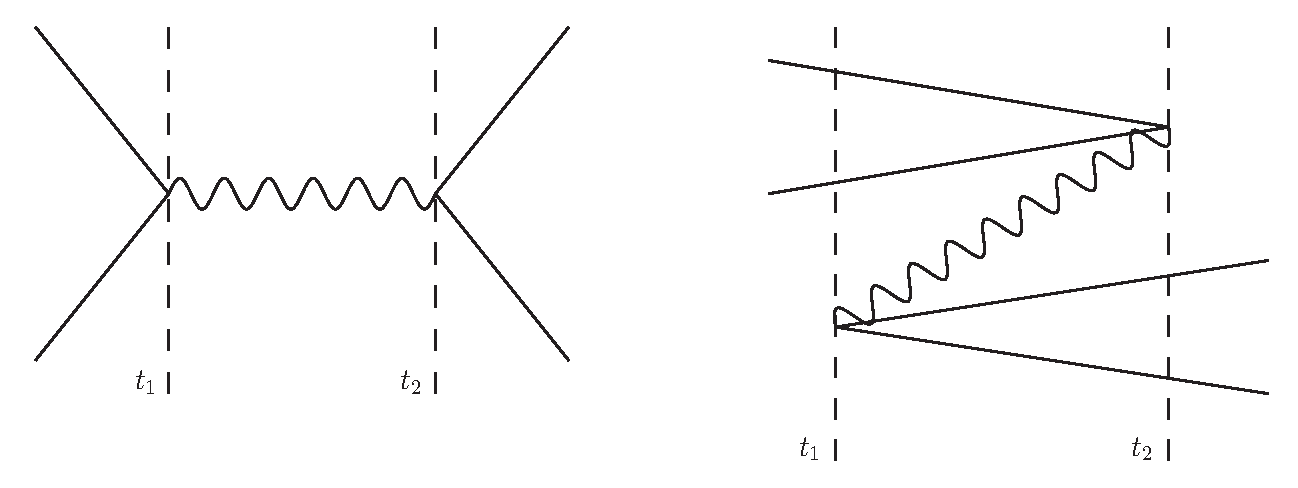
\includegraphics[width=0.4\textwidth]{./proton/1.eps}   
\end{align*}
With energies $E_\gamma, \lambda_\gamma \lessapprox r_{p}$, we can observe proton as a whole or roughly proton structure.

Proton couples to electric charge and we want to know then what is the electric charge distribution of proton $\rho(\pmb{x})$. First we make a couple of assumptions
\begin{itemize}
   \item Non-realistic proton so that it has static charge and is unmovable 
   \item To this scattering process corresponds a cross section (in lab frame)
      \begin{align}
         \dv{\sigma}{\Omega} = \left( \dv{\sigma}{\Omega} \right)_\text{point} \cdot |F(\pmb q)|^2,
      \end{align}
      with $\left( \dv{\sigma}{\Omega} \right)_\text{point}$ the differential cross section of Rutherford scattering and $F(\pmb{q})$ the form factor.
\end{itemize}

Normalization charge distribution 
\begin{align*}
   \int \dd[3]{x} \rho( \pmb x) = 1,
\end{align*}
and $Ze$ overall charge.

Electromagnetic field due to $Ze \rho(\pmb{x})$ and resulting four-potential is $A^\mu = (\rho, 0)$. There is no magnetic field $\pmb{B} = 0$, since the charge is at rest. 
Maxwell equations are
\begin{align*}
   \partial^2 A ^\mu = j^\mu. 
\end{align*}
with  $j^\mu = (\rho, 0)$.

The field is static $\phi(\pmb{x}, t) = \phi(\pmb x)$
\begin{align*}
   \nabla^2 \phi = - Ze \rho(\pmb x).
\end{align*}

The transition amplitude is
\begin{align*}
   T_{fi} &= -i \int \dd[4]{x} j_\mu^{fi} A^\mu,
   \shortintertext{with electron current}
   j_\mu^{fi} &= -e \bar{u}_f \gamma_\mu u_i \euler^{i(p_f - p_i)\cdot x}.
   \shortintertext{Then}
   T_{fi} &= -i 2 \pi \delta (E_f - E_i) ( -e \bar{u}_f \gamma_0 u_i) \int \dd[3]{x} \euler^{i\pmb{q}\cdot \pmb{x}}\phi(\pmb{x}), \\
   \int \dd[3]{x} \euler^{i\pmb{q}\cdot \pmb{x}} \underbrace{\nabla^2 \phi(\pmb{x})}_{-Ze \rho(\pmb{x})} &= - |\pmb{q}|^2 \int \dd[3]{x} \euler^{i\pmb{q} \cdot \pmb{x}}\phi(\pmb x), \\
   \int \dd[3]{x} \euler^{i\pmb{q} \cdot \pmb{x}} \phi(\pmb{x}) &= - \frac{1}{|\pmb{q}|^2} \int \dd[3]{x} \euler^{i \pmb{q} \cdot \pmb{x}} \nabla^2 \phi(\pmb{x}), \\
                                                                &= - \frac{1}{|\pmb{q}|^2} \int \dd[3]{x} \euler^{i\pmb{q} \cdot \pmb{x}} (-Ze) \rho(\pmb{x}),
\end{align*} 
This is just Fourier transformation of $\rho(\pmb x)$. The form factor is defined as
\begin{align}
   F(\pmb{q}) = \int \dd[3]{x} \euler^{i\pmb{q} \cdot \pmb{x}} \rho(\pmb x).
\end{align}

We are looking at scattering off of static charge distribution $A B \rightarrow CD$
\begin{align*}
   T_{fi} &= -i N_A N_B N_C N_D (2\pi)^4 \delta^{(4)}(p_C + p_D - p_A - p_B) \M, \\ 
   W_{fi} &= \frac{|T_{fi}|^2}{T V}, \\
          &= \frac{(2\pi)^4}{V^4} \delta^{4}(p_c + p_D - p_A - p_B)|\M|^2.
\end{align*}

Cross section is defined by
\begin{align}
   \sigma = \frac{W_{fi}}{\text{initial flux}} (\text{number of final states}).
\end{align}
We find
\begin{align}
   \dd{\sigma} = \frac{|T_{fi}|^2}{T} \frac{\dd[3]{k_f}}{(2\pi)^3 2 E_f} \left( \frac{1}{v2E_i} \right),
\end{align}
in which
\begin{align*}
   &\dd[3]{k_f} \delta(E_f - E_i), \\
   =& |\pmb{k}_f|^2 \dd{|\pmb{k}_k|} \dd{\Omega_f} \delta(E_f - E_i), \\
   =& |\pmb{k}_f|E_f \dd{E_f} \delta(E_f - E_i) \dd{\Omega_f}, \\
   =& |\pmb{k}_f| E_{i=f} \dd{\Omega_f}.
\end{align*} 
where
\begin{align*}
   E^2 &= k^2 + m^2, \\
   2 E \dd{E} &= 2 k \dd{k}, \\
   k \dd{k} &= E \dd{E}.
\end{align*}

The spinor structure in final (differential) cross section  is
\begin{align*}
   \frac{1}{2} \sum_{\text{spin}} \left| \bar{u}_f \gamma_0 u_i \right|^2 = 4 E^2 \left(1- v^2 \sin^2\frac{\theta}{2} \right),
\end{align*}
with $\theta$ the scattering angle of electron.

Expressing the momentum transfer $q^2 = (k_i - k_f)^2 $ in terms of $E$, $\theta$, the cross section is
\begin{align}
   \dv{\sigma}{\Omega} &= \frac{(Z\alpha)^2 E^2}{4 k^4 \sin^4 \frac{\theta}{2}} \left(1- v^2 \sin^2 \frac{\theta}{2} \right) |F(\pmb{q})|^2, \\
                       &= \left( \dv{\sigma}{\Omega} \right)_{\text{point}} |F(\pmb{q})|^2.
\end{align}
According to the definition $F(0) = 1$.

With long wavelength or small $|\pmb{q}|$, the exponential is to be expanded
\begin{align*}
   \euler^{i \pmb{q} \cdot\pmb {x}} &= 1 + i \pmb{q} \cdot \pmb{x} - \frac{1}{2} (\pmb{q} \cdot \pmb{x})^2 + \dots, \\
   F(\pmb{q}) &= \int \dd[3]{x} \rho(\pmb{x}) \left( 1 + i \pmb{q}\cdot \pmb{x} - \frac{1}{2} (\pmb{q} \cdot \pmb{x})^2 + \dots \right), \\
              &= 1 - \frac{1}{6} |\pmb{q}|^2 \expval{r^2} + \dots,
\end{align*}
assuming $\rho(\pmb{x}) = \rho(|\pmb{x}|)$. First order term drops out because of symmetry consideration. $\expval{r^2}$ is the mean square radius of charge distribution.

\section{Electron-proton scattering, Proton Form Factor}
Real proton is not static, it can recoil also has spin. Consider again $e\mu$ scattering
\begin{align}
   \eval{\dv{\sigma}{\Omega}}_{\text{lab}} = \frac{\alpha^2}{4 E^4 \sin^4 \frac{\theta}{2}} \frac{E'}{E} \left[ \cos^2 \frac{\theta}{2} - \frac{q^2}{2m_\mu^2} \sin^2 \frac{\theta}{2} \right].
\end{align}
The $E'/E$ is indeed the recoil factor
\begin{align*}
   \frac{E'}{E} = \frac{1}{1 + \frac{2E}{m_\mu } \sin^2 \frac{\theta}{2}}.
\end{align*}

How did calculation proceed?
\begin{align*}
   T_{fi} &= -i \int \dd[4]{x} j_\mu \left( - \frac{1}{q^2} \right) J_p^\mu, \\
   j^\mu &= -e \bar{u}(k') \gamma^\mu u(k) \euler^{i(k'-k)\cdot x}, \\
   J_p^\mu &= e \bar{u}(p')  \left[ \dots  \right]^\mu u(p) \euler^{i (p'-p)\cdot x}.
\end{align*}

$J_p^\mu$ must be a Lorentz four-vector in the form of
\begin{align*}
   \left[ \dots \right]^\mu = F_1(q^2) \gamma^\mu + \frac{\kappa}{2 m_p} F_2 (q^2) i \sigma^{\mu\nu} q_\nu.
\end{align*}
In principle, can also write a term with $\gamma^5$, it leads to parity violation but EM-sector doesn't violate parity. 

So why is this expression the most general form? More in general, one can have
\begin{align*}
   J^\mu = e \bar{u}(p') \left[ \gamma^\mu K_1 + i \sigma^{\mu\nu} (p'-p)_\nu K_2 + i\sigma^{\mu\nu} (p' + p)_\nu K_3 + (p'-p)^\mu K_4 + (p'+p)^\mu K_5 \right] u(p) \euler^{i q \cdot x}.
\end{align*}

Recall Gordon identity
\begin{align}
   \bar{u}_f \gamma^\mu u_i = \frac{1}{2m} \bar{u}_f \left[ (p_f + p_i)^\mu + i \sigma^{\mu\nu} (p_f - p_i)_\nu \right] u_i.
\end{align}
With this identity, we can get rid of term containing $K_5$. For some reasons, $K_3$ term drops out also (second Gordon identity)
\begin{align*}
   J^\mu = e \bar{u}(p) \left[ \gamma^\mu F_1 + \frac{i \kappa}{2 m_p} F_2 \sigma^{\mu\nu} q_\nu + q^\mu F_3 \right] u(p) \euler^{iq\cdot x}.
\end{align*}

Applying current conservation in momentum space $q_\mu J^\mu = 0$. Then
\begin{align*}
   q_\mu J^\mu = e \bar{u}(p') \left[ \slashed{q} F_1 + \frac{i\kappa}{2m_p} F_2 q_\mu \sigma^{\mu\nu} q_\nu + q^2 F_3  \right] u(p) = 0
\end{align*}
The second term drops out using symmetry argument (in $\mu\nu$). The first term drops out using Dirac equation twice. Thus $F_3 = 0$.

Finally, we arrive at the same expression
\begin{align*}
   J^\mu = e \bar{u}(p') \left[ \gamma^\mu F_1 + \frac{i\kappa}{2 m_p} \sigma^{\mu\nu} q_\nu F_2 \right]u(p) \euler^{iqx}.
\end{align*}
Then
\begin{align*}
   \M \sim \left( \frac{-1}{q^2} \right) j_\mu J_p^\mu.
\end{align*}

For long wavelength $q \rightarrow 0$, particle of charge $+e$ and magnetic moment $\frac{(1+\kappa)e}{2 m_p}$
\begin{align*}
   F_1 (0) = 1, \quad F_2 (0) = 1, \quad \kappa \approx 1.79.
\end{align*}

We can do the same experiment on neutron
\begin{align*}
   F_1 (0) = 0, \quad F_2(0) = 1, \quad \kappa \approx -1.91.
\end{align*}

The full differential cross section reads
\begin{align}
   \eval{\dv{\sigma}{\Omega}}_{\text{lab}} = \frac{\alpha^2}{4 E^2 \sin^2 \frac{\theta}{2}} \frac{E'}{E} \left[ (F_1^2 - \frac{\kappa^2 q^2}{4m_p^2}F_2^2) \cos^2 \frac{\theta}{2} - \frac{q^2 }{2m_p^2} (F_1 + \kappa F_2)^2 \sin^2 \frac{\theta}{2} \right].
\end{align}

One can redefine the quantities as
\begin{align}
   G_E &= F_1 + \frac{\kappa q^2}{4 m_p^2} F_2, \\
   G_M &= F_1 + \kappa F_2.
\end{align}

With $ \tau = - \frac{q^2}{4m_p^2} $, the cross section can be rewritten as
\begin{align}
   \eval{\dv{\sigma}{\Omega}}_{\text{lab}} =  \frac{\alpha^2}{4 E^2 \sin^2 \frac{\theta}{2}} \frac{E'}{E} \left[ \frac{G_E^2 + \tau G_M^2 }{1 + \tau} \cos^2 \frac{\theta}{2} + 2 \tau G_M^2 \sin^2 \frac{\theta}{2} \right].
\end{align}

Experimentally
\begin{align*}
   G_E(q^2) \approx \left( 1 - \frac{q^2}{0.71} \right)^{-2}
\end{align*}
with $q^2$ in units of $GeV^2$. The radius can be determined 
\begin{align*}
   \expval{r^2} = 6 \eval{ \left( \dv{G_F(q^2)}{q^2} \right) }_{q^2 = 0} = ( \SI{0.81e-13}{\cm})^2.
\end{align*}
There was discrepancy in determination of proton charge radius, but recently resolved. For more information, check \cite{hammer2019proton}.

%%%%%%%%%%%%%%%%%%%%%%%%%%%%%%%%%%%%%%%%%%%%%%%%%%%%%%%%%%%%%%%%%
% Lecture date: 20-01-21
%%%%%%%%%%%%%%%%%%%%%%%%%%%%%%%%%%%%%%%%%%%%%%%%%%%%%%%%%%%%%%%%%
\section{Inelastic Proton-electron Scattering}
To increase the energy of exchange photon $q^2 = (k - k')^2$, we can increase the energy of the electron
Smaller wavelength means that we can probe substructure of proton. At some point, the quark structure is resolved.
\begin{align*}
   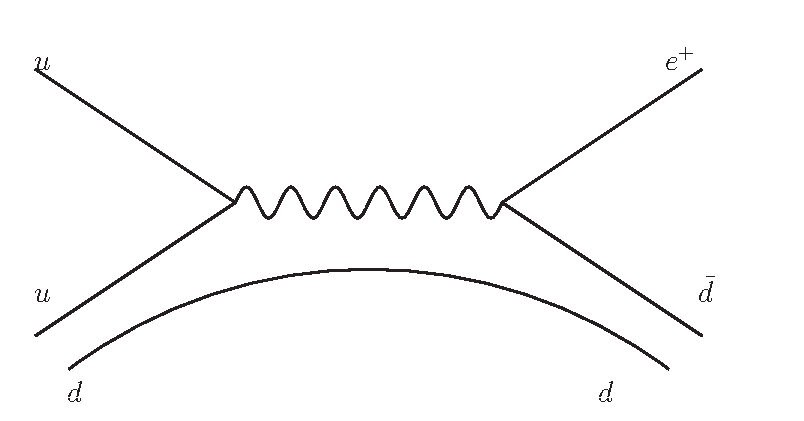
\includegraphics[width=0.3\textwidth]{./proton/2.eps}\\
\end{align*}
At higher energy proton an be excited and/or break up. They are not the same particle as before any more. Thus it is inelastic scattering. 
Denoting the momentum of outgoing particle $p_i$, then the invariant mass is
\begin{align*}
   w^2 = \left( \sum_{i=1}^{N} p_i \right)^2.
\end{align*}

Simplest case is $\Delta^+$-resonance: $e^- p \rightarrow e^- \Delta^+ \rightarrow e^- p \pi^0$. Effectively it is $\gamma^* p \rightarrow \Delta^+ \rightarrow p \pi^0$. This might be relevant in cosmic rays. Partly because of supernova explosion, there are lots of energetic proton going in all directions. Cosmic microwave background provides constant photon distribution to enable this reaction. In this process, the proton loses $\sim 20 \%$ of its energy. Since $M_{\Delta^+} = \SI{1.232}{\giga \eV}$, proton with typical energy $E_p \gtrapprox \SI{10e20}{\eV}$ can take part in multiple this kind of reactions. But there is no known source of proton $E_p > \SI{10e20}{\eV}$ in our galaxy.

Mean free path of a proton with $E \gtrapprox \SI{10e20}{\eV}$ is almost about $50 Mpc$. Next high energy source is further away. Measure energy spectrum of cosmic rays hitting Earth. Should not see any proton above $\SI{10e20}{\eV}$. It is called GZK-cutoff. 

On the Earth, measuring the proton energy is hard because of the shower it produces entering the atmosphere.
There were several groups claiming to detect abnormally high energy protons. But the puzzle has been resolved by Pierre Auger experiment.

Below the dashed line there is no longer a single fermion. We can just use $\bar{u}_p \Gamma u_p$.

In $e\mu$-scattering
\begin{align*}
   \dd{\sigma} \sim L_{\mu\nu}^e \left( L^\text{muon} \right)^{\mu\nu}.
\end{align*}

Here
\begin{align*}
   \dd{\sigma} \sim L^e_{\mu\nu} (H^{\text{had}})^{\mu\nu} = L^e_{\mu\nu} W^{\mu\nu}.
\end{align*}

Write most general tensor for $W^{\mu\nu}$ with $g^{\mu\nu}, p^\mu, q^\mu$. No gamma matrices, since we have separated the fermion parts. Make the ansatz
\begin{align}
   W^{\mu\nu} = - W_1 g^{\mu\nu} + \frac{W_2}{m_p^2} p^\mu p^\nu + \frac{W_4}{m_p^2} q^\mu q^\nu + \frac{W_5}{m_p^2} (p^\mu q^\nu + q^\mu p^\nu).
\end{align}
It is symmetric in $\mu\nu$, because $L^e_{\mu\nu}$ is symmetric in $\mu\nu$ (otherwise it vanishes). $W_3$ is reserved for parity violation. $W_{1,2}$ are not dimensionless, $[W_{1,2}] = -1$.

Current conservation reads
\begin{align*}
   q_\mu W^{\mu\nu} = q_\nu W^{\mu\nu} = 0.
\end{align*}
Plug the general expression in
\begin{align*}
   q_\mu W^{\mu\nu} &= - W_1 q^\nu + \frac{W_2}{m_p^2} q\cdot p p^\nu + \frac{W_5}{m_p^2} \left( p \cdot q q^\nu + q^2 p^\nu \right) + \frac{W_4}{m_p^2} q^2 q^\nu = 0, \\
                    &= q^\nu \left( - W_1 + \frac{W_4}{m_p^2} q^2 + \frac{W_5}{m_p^2} p \cdot q \right) + p^\nu \left( \frac{W_2}{m_p^2} p \cdot q + q^2 \frac{W_5}{m_p^2} \right) = 0.
\end{align*}
Two parts have to vanish individually. From first part we get
\begin{align*}
   W_5 = - \frac{p \cdot q}{q^2} W_2.
\end{align*}
Second part leads to
\begin{align*}
   -W_1 &+ \frac{W_4}{m_p^2} q^2 + \frac{W_5}{m_p^2} p \cdot q = 0, \\
   W_4 &= \left( \frac{p \cdot q}{q^2} \right)^2 W_2 + \frac{m_p^2 }{q^2} W_1.
\end{align*}
The result from first part shall be used here.

So
\begin{align*}
   W^{\mu\nu} = W_1 \left( -g^{\mu\nu} + \frac{q^\mu q^\nu}{q^2} \right) + \frac{W_2}{m_p^2} \left( p^\mu - \frac{p\cdot q}{q^2} q^\mu \right) \left( p^\nu - \frac{p\cdot q}{q^2} q^\nu \right).
\end{align*}

Define
\begin{align}
   \nu = \frac{p \cdot q}{m_p}.
\end{align}
then $W_1$ and $W_2$ can be expresses by $\nu$ and $q^2$
\begin{align*}
   W_1 = W_1 (q^2, \nu), \quad W_2 = W_2 (q^2 , \nu).
\end{align*}

By momentum conservation $W^2 = (p + q)^2 = m_p^2 + 2 m_p \nu + q^2 $.

Define 
\begin{align}
   x &= - \frac{q^2}{2 p \cdot q} = -\frac{q^2}{2 m_p \nu}, \\
   y &= \frac{p \cdot q }{p \cdot k}.
\end{align}
They are dimensionless. 

In $e p \rightarrow e X$, $0 \leq x \leq 1$ and  $0 \leq y \leq 1$.  Proton is at rest, $p = (m_p, 0)$.
\begin{align*}
   q = k - k',\quad q^0 = E - E'.
\end{align*}
Thus 
\begin{align*}
   y &= \frac{m_p (E-E')}{m_p E} = \frac{E-E'}{E},  \\
   \nu &= \frac{p \cdot q}{m_p} = \frac{m_p (E- E')}{m_p} = E- E'.
\end{align*}

Now, lets get back to cross section
\begin{align*}
   L^{e \, \mu\nu} W_{\mu\nu} &= 4 W_1 (k \cdot k') + \frac{2 W_2}{m_p^2} \left[ 2 (p\cdot k )(p \cdot k') - m_p^2 (k\cdot k') \right], \\
   \shortintertext{go to the lab frame}
                              &= 4 E E' \left[ \cos^2 \frac{\theta}{2} W_2 (\nu,  q^2) + \sin^2 \frac{\theta}{2} 2 W_1 (\nu, q^2) \right].
\end{align*}
The cross section is then
\begin{align*}
   \dd{\sigma} &= \frac{1}{ 4 \left[ (k \cdot p)^2 - m_e^2 m _p^2 \right]} \left[ \frac{e^4}{q^4} L^{e\, \mu\nu} W_{\mu\nu} 4 \pi m_p \right] \frac{\dd[3]{k'}}{ 2E' (2\pi)^3} \\
   \eval{\frac{\dd{\sigma}}{\dd{E'}\dd{\Omega}}}_{\text{\lab}} &= \frac{\alpha^2}{4 E^2 \sin^2 \frac{\theta}{2}} \left\{ W_2 (\nu, q^2) \cos^2 \frac{\theta}{2} + 2 W_1 (\nu, q^2) \sin^2 \frac{\theta}{2} \right\}
\end{align*}
Measurement of $W_{1,2}$ to learn about high energy $ep$-interaction. We can use interaction of electron and point-like particle (e.g.~muon) and compare it to the measured $W_{1,2}$. It should go to in the limit where the "quarks" are resolved.

\paragraph{Summary}
\begin{align}
   \frac{\dd{\sigma}}{\dd{E'}\dd{\Omega}} = \frac{4 \alpha^2 E^2 }{q^2 } \cdot A
\end{align}

\begin{itemize}
   \item Electron-muon scattering
      \begin{align}
         A_{e\mu \rightarrow e \mu} = \left( \cos^2 \frac{\theta}{2} - \frac{q^2}{2 m^2} \sin^2 \frac{\theta}{2} \right) \delta(\nu + \frac{q^2}{m})
      \end{align}
      so $\nu$ and $q^2$ are not independent.
   \item Electron-proton scattering with low energy
      \begin{align}
         A_{e p \rightarrow e p} = \left( \frac{G_E^2 + \tau G_M^2 }{1 + \tau} \cos^2 \frac{\theta}{2} + 2 \tau G_M^2 \sin^2 \frac{\theta}{2} \right) \delta(\nu + \frac{q^2}{2m} )
      \end{align}
      with $\tau = -\frac{q^2}{4 m_p^2}$.
   \item Electron-proton scattering with high energy
      \begin{align}
         A_{ep \rightarrow e X} = W_2 (\nu, q^2) \cos^2 \frac{\theta}{2} + 2 W_1 (\nu, q^2) \sin^2 \frac{\theta}{2}
      \end{align}
\end{itemize}

In (a) and (b), we can integrate $\delta$-function to get differential cross section.
